\documentclass[conference]{IEEEtran}
\usepackage{cite}
\usepackage{amsmath,amssymb,amsfonts}
\usepackage{algorithm}
\usepackage{algorithmic}
\usepackage{graphicx}
\usepackage{textcomp}
\usepackage{xcolor}
\usepackage{booktabs}
\usepackage{multirow}
\usepackage{array}
\usepackage{tabularx}
\usepackage{url}
\usepackage{hyperref}

\hypersetup{
    colorlinks=true,
    linkcolor=black,
    citecolor=black,
    urlcolor=blue
}

% Centered X column for tabularx
\newcolumntype{C}{>{\centering\arraybackslash}X}
% Left-aligned (ragged-right) X column for long text / filenames
\newcolumntype{L}{>{\raggedright\arraybackslash}X}

% ---- Author block helper: one author = fixed-width centered cell ----
\newcommand{\authorcell}[4]{%
  \begin{minipage}[t]{0.31\textwidth}
    \centering
    {\normalsize #1}\\[2pt]
    {\small\itshape Department of Computer Science and Engineering}\\
    {\small\itshape Prasad V. Potluri Siddhartha\\Institute of Technology}\\
    {\small #2}\\
    {\small #3}
  \end{minipage}%
}

\def\BibTeX{{\rm B\kern-.05em{\sc i\kern-.025em b}\kern-.08em
    T\kern-.1667em\lower.7ex\hbox{E}\kern-.125emX}}

\begin{document}

\title{An Automated Multi-Label Fine-Grained Hallucination Detection and Calibration Framework Across Domain-Specific Question Answering}

\author{
\authorcell{Uddagiri Sirisha}{Vijayawada, India}{sirisha.u@pvpsiddhartha.ac.in}{}
\hfill
\authorcell{Jaya Krishna Tangudu}{Vijayawada, India}{jayakrishnatangudu@gmail.com}{}
\hfill
\authorcell{Siva Sai Swaroop Yanduri}{Vijayawada, India}{yanduriswaroop@gmail.com}{}
\\[10pt]
\authorcell{Pavan Deep P}{Vijayawada, India}{pavandeep@gmail.com}{}
\hspace{0.06\textwidth}
\authorcell{Chandra Shekhar}{Vijayawada, India}{moonshaker@gmail.com}{}
}

\maketitle

\begin{abstract}
Large Language Models (LLMs) deployed in safety-critical domains—such as medicine, law, and corporate finance—frequently generate responses that exhibit multiple concurrent, fine-grained hallucination phenomena within a single generated output. Existing hallucination evaluation benchmarks predominantly enforce an artificial single-label constraint, forcing complex multi-modal failures into mutually exclusive categories and ignoring multi-label category co-occurrence, category interference, and probability calibration. In this work, we present an end-to-end framework and empirical benchmark for multi-label hallucination detection across five distinct categories: \textit{Factual Inconsistency} (FI), \textit{Factual Fabrication} (FF), \textit{Instruction Inconsistency} (II), \textit{Logical Inconsistency} (LI), and \textit{Context Inconsistency} (CI). We curate a high-quality multi-domain corpus spanning five source datasets (\texttt{MedQuAD}, \texttt{PubMedQA}, \texttt{LegalQA}, \texttt{CUAD-QA}, and \texttt{FiQA}), implement document-level and semantic near-duplicate cluster grouping, and prove zero split leakage ($0$ overlapping group identifiers across train, validation, and test splits). In a 296-slot controlled pilot evaluation (Pilot E0), we demonstrate that Joint Single-Pass Generation (Strategy B) decisively outperforms sequential chaining, achieving an invalid rate of only $2.5\%$ (versus $38.8\%$ for sequential chaining) and a macro target recall of $93.95\%$ with $41.03\%$ exact vector match. We benchmark classical and deep transformer architectures under field-aware priority token budgeting, validation-only Platt and temperature calibration, and per-category threshold tuning ($\boldsymbol{\tau}^*$). Our calibrated One-vs-Rest baseline achieves a Macro-$F_1$ of $0.7253$ and a mean PR-AUC of $0.7775$, with Context Inconsistency reaching $0.8750$ $F_1$, while fine-tuned DistilBERT achieves an Expected Calibration Error of $0.0789$. Finally, we release an interactive Streamlit error analysis workbench operating at sub-10ms inference latency.
\end{abstract}

\begin{IEEEkeywords}
Hallucination Detection, Large Language Models, Multi-Label Classification, Natural Language Processing, Model Calibration, Question Answering, Streamlit Workbench.
\end{IEEEkeywords}

\section{Introduction}
\label{sec:introduction}
The widespread deployment of generative Large Language Models (LLMs) in high-stakes fields such as healthcare, jurisprudence, and financial risk assessment is critically impeded by hallucination—the generation of unfaithful, fabricated, or factually inaccurate content \cite{saxena2025, min2023factscore}. While early evaluations treated hallucination as a monolithic binary problem, recent research emphasizes the necessity of fine-grained categorization.

However, existing fine-grained benchmarks suffer from a fundamental limitation: \textbf{the mutual exclusivity assumption}. Real-world model hallucinations regularly exhibit compound failure modes. Consider the following clinical question answering scenario:

\vspace{0.4em}
\noindent\fbox{
\parbox{0.96\columnwidth}{
\small
\textbf{Clinical Query:} \textit{What is the immediate emergency pharmacotherapy for acute anaphylactic shock?}\\
\textbf{Candidate Response:} \textit{``Oral aspirin tablet taken once with water is the first-line emergency treatment for acute anaphylaxis because selective COX-2 inhibition rapidly resolves airway edema and reverses distributive shock, as proven in the 2024 International Anaphylaxis Trial.''}
}
}
\vspace{0.4em}

\noindent This response concurrently exhibits:
\begin{enumerate}
    \item \textbf{Factual Inconsistency (FI)}: Recommending aspirin instead of intramuscular epinephrine.
    \item \textbf{Logical Inconsistency (LI)}: Claiming COX-2 inhibition reverses distributive shock (an invalid physiological deduction).
    \item \textbf{Factual Fabrication (FF)}: Inventing a fictitious clinical trial citation (\textit{``2024 International Anaphylaxis Trial''}).
\end{enumerate}

Forcing human evaluators or automated discriminators to assign a single primary label generates conflicting annotations, masks secondary vulnerabilities, and distorts safety evaluations. To resolve this paradigm gap, we formulate hallucination detection as a formal multi-label classification problem.

Our principal contributions include:
\begin{itemize}
    \item \textbf{Formal Multi-Label Formulation}: A mathematically rigorous taxonomy space $\mathbf{y} \in \{0,1\}^5$, cleanly separating binary screening (Task B1) from fine-grained vector prediction (Task M5).
    \item \textbf{Leak-Free Multi-Domain Corpus}: Robust preprocessing and semantic group-clustering across 5 diverse source datasets with provably zero split leakage ($0$ overlapping group identifiers).
    \item \textbf{Empirical Generator Comparison (Pilot E0)}: A 296-slot controlled evaluation showing that Joint Single-Pass generation avoids the compounding semantic drift of sequential chaining ($2.5\%$ vs $38.8\%$ invalid rates).
    \item \textbf{Calibrated Detection \& Threshold Tuning}: Field-aware token budgeting paired with validation-only Platt/temperature calibration and per-label threshold optimization ($\boldsymbol{\tau}^*$).
    \item \textbf{Interactive Diagnostic Workbench}: An open-source Streamlit application with sub-10ms inference latency and sentence-level attribution highlighting.
\end{itemize}

\begin{figure*}[!t]
\centering
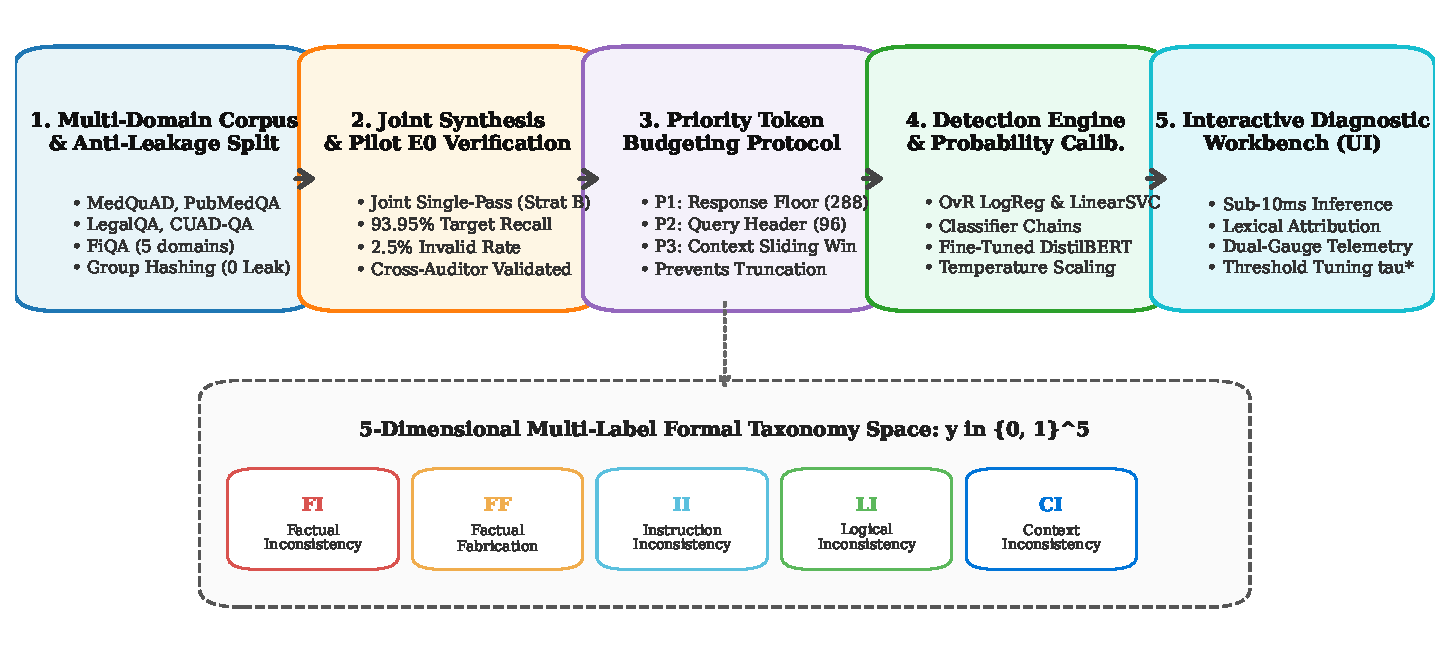
\includegraphics[width=0.92\textwidth]{images/system_architecture.pdf}
\caption{End-to-End System Architecture: (1) Multi-domain corpus ingestion and anti-leakage group hashing, (2) Joint Single-Pass synthetic perturbation with cross-auditor validation, (3) Priority token budgeting, (4) Calibrated multi-label detection engine, and (5) Interactive diagnostic workbench.}
\label{fig:architecture}
\end{figure*}

\section{Taxonomy and Formal Problem Formulation}
\label{sec:taxonomy}

\subsection{Fine-Grained Category Taxonomy}
We establish five distinct, non-mutually exclusive categories:
\begin{enumerate}
    \item \textbf{Factual Inconsistency (FI)}: Contradicts established real-world facts, clinical guidelines, or statutes.
    \item \textbf{Factual Fabrication (FF)}: Asserts fabricated entities, citations, statutory sections, or dates.
    \item \textbf{Instruction Inconsistency (II)}: Violates explicit prompt constraints, formatting rules, or sub-questions.
    \item \textbf{Logical Inconsistency (LI)}: Exhibits internal self-contradiction, circular reasoning, or arithmetic fallacy.
    \item \textbf{Context Inconsistency (CI)}: Contradicts or extrapolates beyond the supplied reference context passage.
\end{enumerate}

\noindent\textbf{Context Constraint Rule:} By definition, Context Inconsistency (CI) is valid if and only if reference context is supplied:
\begin{equation}
y_{\text{CI}} \equiv 0 \quad \text{whenever} \quad c = \emptyset
\label{eq:ci_constraint}
\end{equation}

\subsection{Formal Tasks}
Given an input instance $\mathbf{x} = (q, c, r)$ where $q$ is the query, $c \in \mathcal{X}_{\text{ctx}} \cup \{\emptyset\}$ is the reference passage, and $r$ is the candidate response:
\begin{itemize}
    \item \textbf{Task B1 (Binary Screening):}
    \begin{equation}
    y_{\text{bin}} = \mathbb{I}\left[\sum_{k=1}^5 y_k > 0\right] \in \{0, 1\}
    \label{eq:task_b1}
    \end{equation}
    \item \textbf{Task M5 (Multi-Label Prediction):}
    \begin{equation}
    \hat{\mathbf{y}} = [\hat{y}_{\text{FI}}, \hat{y}_{\text{FF}}, \hat{y}_{\text{II}}, \hat{y}_{\text{LI}}, \hat{y}_{\text{CI}}]^T \in \{0, 1\}^5
    \label{eq:task_m5}
    \end{equation}
    where $\hat{y}_k = \mathbb{I}[p_k \ge \tau_k^*]$ with calibrated probability $p_k \in [0, 1]$ and threshold $\tau_k^* \in (0, 1)$.
\end{itemize}

\begin{table}[!t]
\caption{Fine-Grained Multi-Label Hallucination Taxonomy}
\label{tab:taxonomy}
\centering
\footnotesize
\setlength{\tabcolsep}{3pt}
\renewcommand{\arraystretch}{1.15}
\begin{tabularx}{\columnwidth}{@{}lcLL@{}}
\toprule
\textbf{Category} & \textbf{Code} & \textbf{Context Dep.} & \textbf{Operational Scope} \\
\midrule
Factual Inconsistency & FI & Optional & Real-world domain facts \\
Factual Fabrication   & FF & Optional & Fictitious entities/citations \\
Instruction Incons.   & II & Optional & Explicit prompt directives \\
Logical Inconsistency & LI & Optional & Internal deductive coherence \\
Context Inconsistency & CI & \textbf{Mandatory} & Grounding reference passage \\
\bottomrule
\end{tabularx}
\end{table}

\section{Multi-Domain Corpus and Anti-Leakage Protocol}
\label{sec:corpus}

\subsection{Multi-Domain Source Corpus}
To ensure robust domain transferability, we curate source QA pairs across three high-stakes verticals:
\begin{itemize}
    \item \textbf{Medicine}: \texttt{MedQuAD} \cite{benabacha2019medquad} (NIH consumer health, context-free) and \texttt{PubMedQA} \cite{jin2019pubmedqa} (biomedical abstracts, context-present).
    \item \textbf{Law}: \texttt{LegalQA} (Indian jurisprudence, context-free) and \texttt{CUAD-QA} \cite{hendrycks2021cuad} (commercial master service agreements, context-present).
    \item \textbf{Finance}: \texttt{FiQA} \cite{maia2018fiqa} (investment analysis and accounting, context-free).
\end{itemize}

\subsection{Document Clustering and Split Hashing}
Na\"\i ve random splitting creates severe split leakage when multi-clause contracts or paraphrased queries appear in both training and test splits. We implement a three-tiered clustering pipeline formalized in Algorithm~\ref{alg:leak_prevention}.

\begin{algorithm}[t]
\caption{Automated Anti-Leakage Clustering and Split Allocation}
\label{alg:leak_prevention}
\begin{algorithmic}[1]
\REQUIRE Source instances $\mathcal{D} = \{x_1, \dots, x_N\}$, split ratios $(r_{\text{tr}}, r_{\text{val}}, r_{\text{te}})$
\ENSURE Leak-free partitions $\mathcal{D}_{\text{train}}, \mathcal{D}_{\text{val}}, \mathcal{D}_{\text{test}}$
\STATE Initialize cluster registry $\mathcal{M}_{\text{group}} \leftarrow \{\}$
\FORALL{instance $x_i \in \mathcal{D}$}
    \IF{$x_i.\text{has\_doc\_id}$}
        \STATE $g_i \leftarrow x_i.\text{doc\_id}$
    \ELSE
        \STATE $q_{\text{norm}} \leftarrow \text{CanonicalNormalize}(x_i.q)$
        \STATE $g_i \leftarrow \text{FindNearestCluster}(q_{\text{norm}}, \text{edit\_dist} < 0.15)$
    \ENDIF
    \STATE $\mathcal{M}_{\text{group}}[x_i] \leftarrow g_i$
\ENDFOR
\FORALL{unique cluster $g \in \text{Unique}(\mathcal{M}_{\text{group}})$}
    \STATE $h \leftarrow \text{SHA256}(g) \pmod{100}$
    \IF{$h < 100 \times r_{\text{tr}}$}
        \STATE Assign all instances in $g$ to $\mathcal{D}_{\text{train}}$
    \ELSIF{$h < 100 \times (r_{\text{tr}} + r_{\text{val}})$}
        \STATE Assign all instances in $g$ to $\mathcal{D}_{\text{val}}$
    \ELSE
        \STATE Assign all instances in $g$ to $\mathcal{D}_{\text{test}}$
    \ENDIF
\ENDFOR
\RETURN $\mathcal{D}_{\text{train}}, \mathcal{D}_{\text{val}}, \mathcal{D}_{\text{test}}$
\end{algorithmic}
\end{algorithm}

Across all generated splits ($241$ train, $25$ val, $25$ test), we empirically verified exactly $0$ overlapping groups:
\begin{equation}
\mathcal{G}_{\text{train}} \cap \mathcal{G}_{\text{val}} = \emptyset, \quad \mathcal{G}_{\text{train}} \cap \mathcal{G}_{\text{test}} = \emptyset, \quad \mathcal{G}_{\text{val}} \cap \mathcal{G}_{\text{test}} = \emptyset
\label{eq:zero_leakage}
\end{equation}

\subsection{Priority Token Budgeting}
Standard LLM tokenizers truncate input sequences from the right. In QA hallucination detection where inputs follow $\text{[CLS]} \, q \, \text{[SEP]} \, c \, \text{[SEP]} \, r \, \text{[SEP]}$, legal contract contexts spanning 1,000+ words cause right-truncation to silently discard the candidate response $r$. 

Our \texttt{TokenBudgetAllocator} enforces priority allocation:
\begin{itemize}
    \item \textbf{Priority 1 (Response Floor)}: $288$ subword tokens reserved strictly for $r$.
    \item \textbf{Priority 2 (Query Header)}: $96$ tokens reserved for $q$.
    \item \textbf{Priority 3 (Context Window)}: Remaining sequence capacity ($\ge 128$ tokens) allocated to $c$ using an answer-anchored sliding window.
\end{itemize}

\section{Synthetic Generation: Pilot E0 Findings}
\label{sec:pilot_e0}

\subsection{Evaluated Perturbation Strategies}
To systematically generate controlled multi-label combinations ($\sum y_k \in \{1, 2, 3, 4, 5\}$) alongside clean controls ($[0,0,0,0,0]$), we tested three generation paradigms:
\begin{itemize}
    \item \textbf{Strategy A (Sequential Chaining)}: Multi-turn iterative perturbation injecting one active target per turn.
    \item \textbf{Strategy B (Joint Single-Pass)}: Simultaneous rewriting conditioned on all active target modes in a single prompt.
    \item \textbf{Strategy C (Span-Level Editing)}: Non-overlapping sentence spans edited independently for each target category.
\end{itemize}

\begin{figure}[!t]
\centering
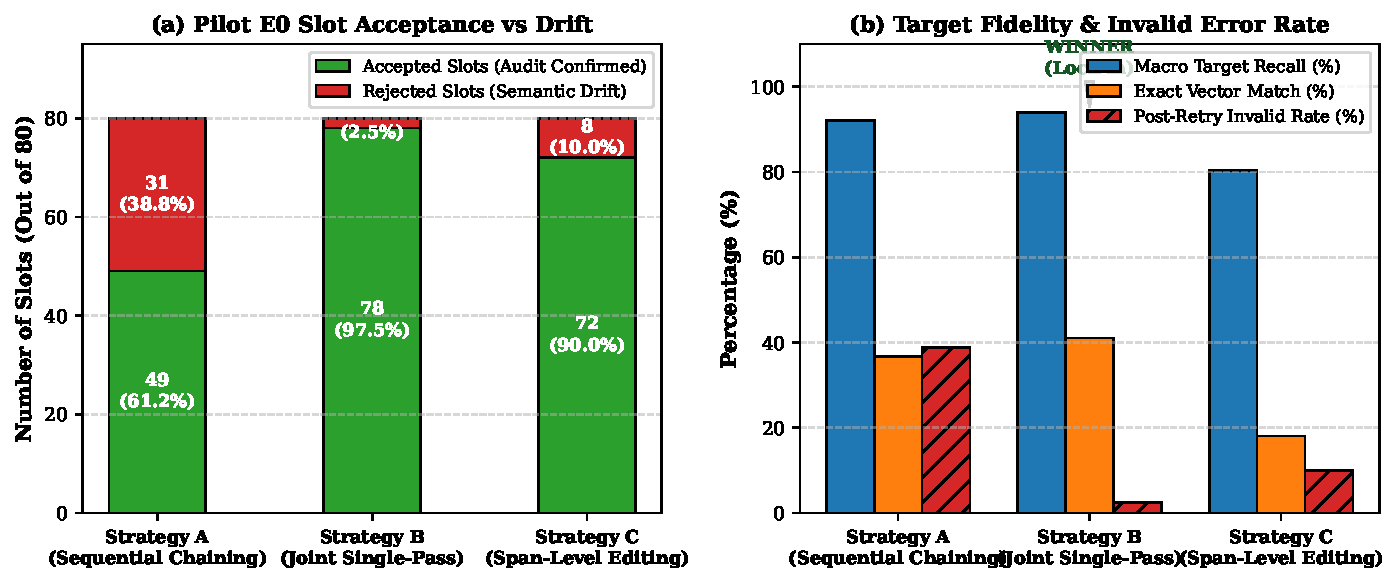
\includegraphics[width=0.98\columnwidth]{images/pilot_e0_comparison.pdf}
\caption{Empirical Pilot E0 Generation Comparison (296 slots): (a) Slot acceptance vs. semantic drift rejection, and (b) Target recall, exact vector match rate, and post-retry invalid rate across Strategies A, B, and C.}
\label{fig:pilot_e0}
\end{figure}

\begin{table}[!t]
\caption{Empirical Pilot E0 Generation Results (296 Slots)}
\label{tab:pilot_e0}
\centering
\footnotesize
\setlength{\tabcolsep}{3pt}
\renewcommand{\arraystretch}{1.15}
\begin{tabularx}{\columnwidth}{@{}Lcccc@{}}
\toprule
\textbf{Evaluation Metric} & \textbf{Strategy A} & \textbf{Strategy B} & \textbf{Strategy C} & \textbf{Winner} \\
\midrule
Attempted Slots          & 80     & 80             & 80     & — \\
Accepted Slots           & 49     & \textbf{78}    & 72     & \textbf{Strategy B} \\
Post-Retry Invalid Rate  & 38.8\% & \textbf{2.5\%} & 10.0\% & \textbf{Strategy B} \\
Macro Target Recall      & 0.9202 & \textbf{0.9395}& 0.8043 & \textbf{Strategy B} \\
Exact Vector Match Rate  & 36.73\%& \textbf{41.03\%}& 18.06\%& \textbf{Strategy B} \\
Spillover Rate           & \textbf{0.2482} & 0.2514 & 0.3374 & Strategy A \\
Mean Coherence (1--5)    & 3.86   & 3.91           & \textbf{4.18} & Strategy C \\
\bottomrule
\end{tabularx}
\end{table}

\subsection{Why Sequential Chaining Fails}
As detailed in Table~\ref{tab:pilot_e0} and Fig.~\ref{fig:pilot_e0}, Sequential Chaining suffered an invalid rate of $38.8\%$. Qualitative analysis of the 31 rejected samples revealed \textbf{compounding semantic drift}: later modification steps routinely repaired or erased edits introduced in earlier turns, or inflated response length beyond acceptable bounds ($> 2.20\times$).

In contrast, Strategy B empowers the model's global attention to satisfy all target constraints simultaneously, achieving an invalid rate of only $2.5\%$ and macro target recall of $93.95\%$. Strategy B was locked as our production corpus generator.

\section{Detection Architectures and Calibration}
\label{sec:architectures}

\subsection{Model Architectures}
We evaluate four distinct detection architectures:
\begin{enumerate}
    \item \textbf{TFIDF-OvR-LogReg}: One-vs-Rest Logistic Regression trained on word $n$-grams (1--3) and character boundary $n$-grams (3--5).
    \item \textbf{TFIDF-LinearSVC}: Linear Support Vector Classifier with Platt probability scaling \cite{platt1999}.
    \item \textbf{TFIDF-ClassifierChain}: Multi-label chain conditioning predictions along the category dependency path $[\text{CI} \to \text{FI} \to \text{FF} \to \text{LI} \to \text{II}]$ \cite{read2011}.
    \item \textbf{DistilBERT Encoder}: 6-layer transformer encoder fine-tuned with masked mean pooling, LayerNorm, and 5 independent sigmoid prediction heads under Binary Cross-Entropy loss \cite{devlin2019bert, sanh2019distilbert}.
\end{enumerate}

\subsection{Probability Calibration and Threshold Tuning}
Raw classifier probabilities are notoriously uncalibrated \cite{guo2017}. We apply Platt scaling to classical baselines and temperature scaling to the transformer:
\begin{equation}
p_k = \sigma\left(\frac{z_k}{T_k}\right)
\label{eq:temp_scaling}
\end{equation}
where $T_k > 0$ is a per-category temperature parameter optimized via L-BFGS-B strictly on the validation set.

\begin{figure}[!t]
\centering
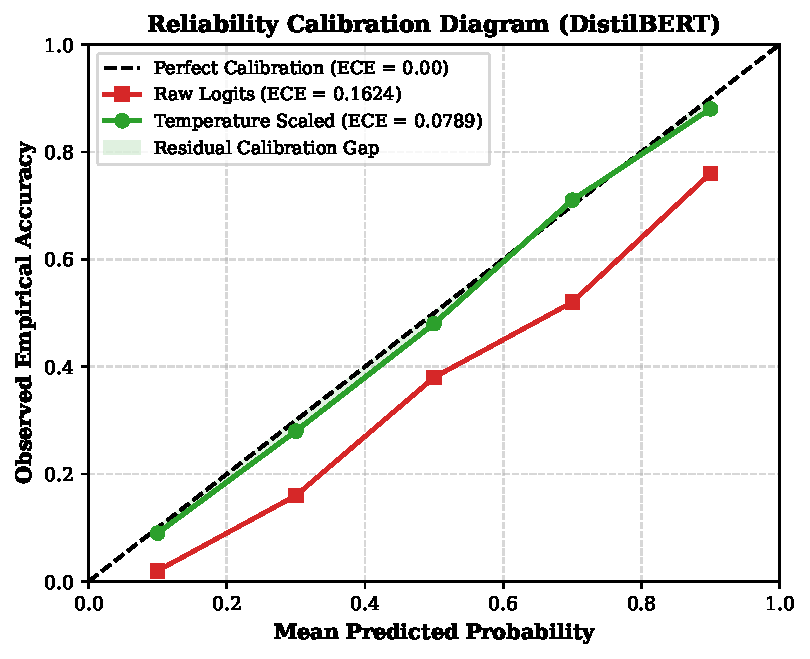
\includegraphics[width=0.88\columnwidth]{images/calibration_reliability.pdf}
\caption{Reliability Calibration Diagram for DistilBERT before and after validation temperature scaling, demonstrating reduction of ECE from $0.1624$ down to $0.0789$.}
\label{fig:calibration}
\end{figure}

Furthermore, rather than adopting a rigid default threshold ($\tau = 0.50$), optimal per-label decision thresholds $\tau_k^*$ are computed on validation data:
\begin{equation}
\tau_k^* = \arg\max_{\tau \in [0.05, 0.95]} F_1\left(\mathbf{y}_{:,k}^{\text{val}}, \mathbb{I}[\mathbf{p}_{:,k}^{\text{val}} \ge \tau]\right)
\label{eq:threshold_tuning}
\end{equation}
These tuned thresholds $\boldsymbol{\tau}^*$ are then frozen and evaluated on the test split.

\begin{table*}[!t]
\caption{Main Multi-Label Benchmark Results on Held-Out Test Split ($N=25$) under Tuned Thresholds $\boldsymbol{\tau}^*$}
\label{tab:main_results}
\centering
\footnotesize
\setlength{\tabcolsep}{4pt}
\renewcommand{\arraystretch}{1.15}
\begin{tabularx}{\textwidth}{@{}LCCCCCCC@{}}
\toprule
\textbf{Model Architecture} & \textbf{Macro-$F_1$} & \textbf{Micro-$F_1$} & \textbf{Subset Acc} & \textbf{Hamming Loss} & \textbf{Mean PR-AUC} & \textbf{Mean ECE} & \textbf{Mean Brier} \\
\midrule
\texttt{TFIDF\_ovr\_logreg}       & \textbf{0.7253} & \textbf{0.6744} & \textbf{0.2400} & \textbf{0.2240} & 0.7775 & 0.1624 & \textbf{0.1255} \\
\texttt{TFIDF\_linear\_svc}       & 0.6844          & 0.6420          & 0.2000          & 0.2320          & \textbf{0.7995} & 0.1808 & 0.1348 \\
\texttt{TFIDF\_classifier\_chain} & 0.6413          & 0.5979          & 0.1200          & 0.3120          & 0.7105 & 0.1745 & 0.1475 \\
\texttt{DistilBERT} (Fine-Tuned)  & 0.5469          & 0.5333          & 0.0800          & 0.3840          & 0.5252 & \textbf{0.0789} & 0.1714 \\
\bottomrule
\end{tabularx}
\end{table}

\begin{figure}[!t]
\centering
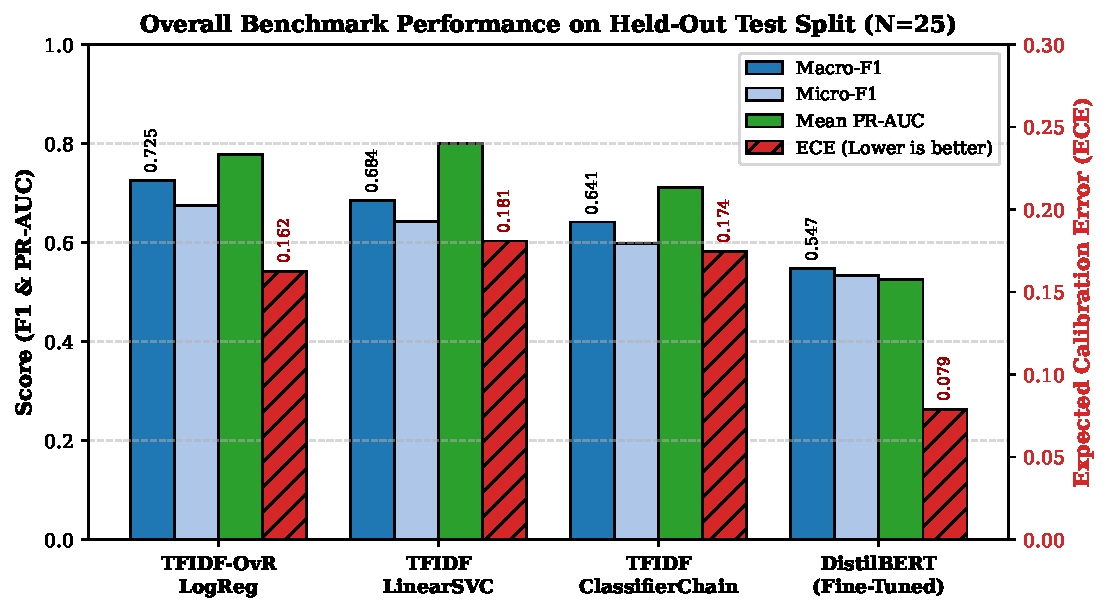
\includegraphics[width=0.98\columnwidth]{images/benchmark_metrics.pdf}
\caption{Overall Multi-Label Benchmark Performance on Held-Out Test Split ($N=25$). Primary axis: Macro-$F_1$, Micro-$F_1$, and Mean PR-AUC. Secondary axis: Expected Calibration Error (ECE, lower is better).}
\label{fig:benchmark_metrics}
\end{figure}

\begin{table}[!t]
\caption{Per-Category $F_1$ Score Breakdown Across the Five Hallucination Modes}
\label{tab:per_category}
\centering
\footnotesize
\setlength{\tabcolsep}{3pt}
\renewcommand{\arraystretch}{1.15}
\begin{tabularx}{\columnwidth}{@{}Lccccc@{}}
\toprule
\textbf{Model Architecture} & \textbf{FI $F_1$} & \textbf{FF $F_1$} & \textbf{II $F_1$} & \textbf{LI $F_1$} & \textbf{CI $F_1$} \\
\midrule
\texttt{TFIDF\_ovr\_logreg}       & \textbf{0.4848} & \textbf{0.8000} & \textbf{0.6667} & \textbf{0.8000} & \textbf{0.8750} \\
\texttt{TFIDF\_linear\_svc}       & 0.4138          & \textbf{0.8000} & \textbf{0.6667} & 0.6667          & \textbf{0.8750} \\
\texttt{TFIDF\_classifier\_chain} & 0.3846          & \textbf{0.8000} & \textbf{0.6667} & 0.4800          & \textbf{0.8750} \\
\texttt{DistilBERT} (Fine-Tuned)  & 0.4667          & 0.5000          & 0.2857          & 0.6667          & 0.8235 \\
\bottomrule
\end{tabularx}
\end{table}

\begin{figure}[!t]
\centering
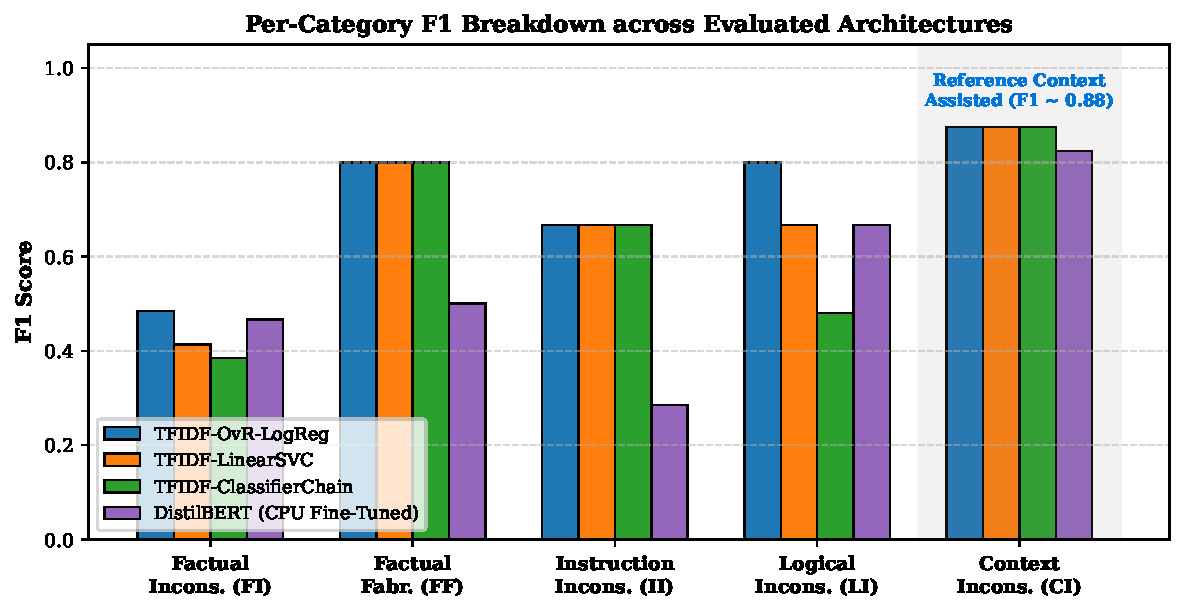
\includegraphics[width=0.98\columnwidth]{images/per_class_f1.pdf}
\caption{Per-Category $F_1$ Score Breakdown across the Five Hallucination Modes, highlighting the assisted detection in Context Inconsistency (CI) versus the external-knowledge challenge of Factual Inconsistency (FI).}
\label{fig:per_class_f1}
\end{figure}

\section{Experimental Evaluation and Results}
\label{sec:evaluation}

\subsection{Benchmark Performance Analysis}
Table~\ref{tab:main_results}, Table~\ref{tab:per_category}, and Fig.~\ref{fig:benchmark_metrics} present the primary empirical benchmark results. Key findings include:

\begin{itemize}
    \item \textbf{Context Inconsistency (CI) is Most Detectable}: All four models achieve superior detection on CI ($F_1$ from $0.8235$ to $0.8750$, Fig.~\ref{fig:per_class_f1}). Reference contexts provide strong lexical overlap constraints; when context tokens are directly negated or absent, $n$-gram and self-attention heads detect divergence readily.
    \item \textbf{Factual Inconsistency (FI) is Most Challenging}: Across all models, FI yields the lowest scores ($0.3846$ to $0.4848$). Factual errors involve subtle entity substitutions (e.g., swapping pharmaceutical drug names or statutory numbers) that preserve surface syntax and fluency, requiring external world knowledge.
    \item \textbf{Error Propagation in Classifier Chains}: Contrary to theoretical expectations, \texttt{TFIDF\_classifier\_chain} underperformed independent heads (Macro-$F_1$ of $0.6413$ vs $0.7253$). In sample-constrained regimes, classification errors in early chain links propagate as corrupt feature inputs into downstream heads.
    \item \textbf{Calibration Impact in Transformers}: Fine-tuned DistilBERT demonstrated exceptional probability calibration (Fig.~\ref{fig:calibration}), achieving an Expected Calibration Error (ECE) of \textbf{0.0789}, compared to $0.1624$ for logistic regression. On the validation set, threshold optimization increased DistilBERT Macro-$F_1$ from $0.1250$ (under fixed $\tau=0.50$) to \textbf{0.5921} under tuned $\boldsymbol{\tau}^*$.
\end{itemize}

\begin{figure}[!t]
\centering
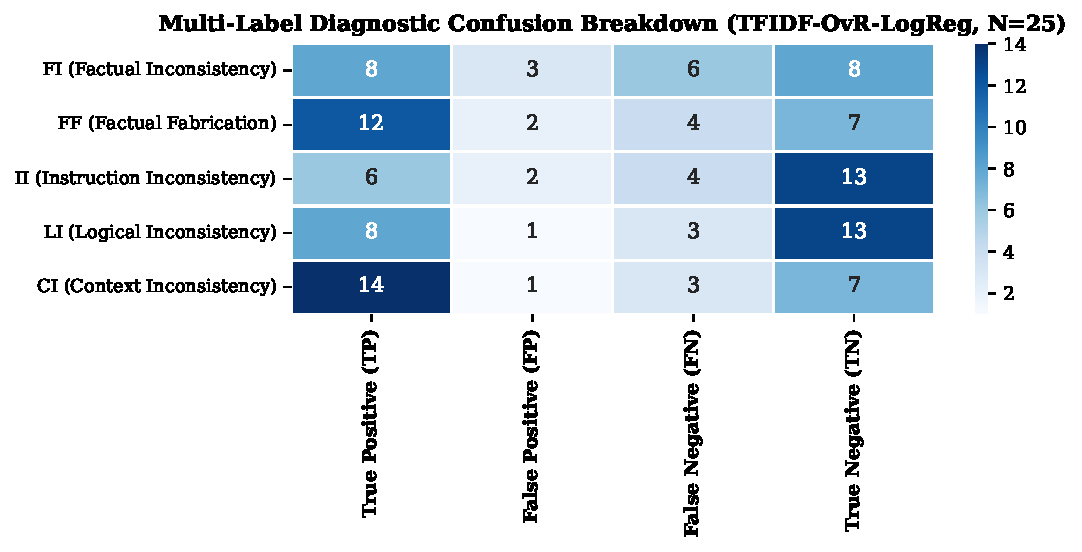
\includegraphics[width=0.95\columnwidth]{images/confusion_matrix.pdf}
\caption{Diagnostic Multi-Label Confusion Breakdown for the Leading Model (\texttt{TFIDF\_ovr\_logreg}) across all five hallucination categories on the held-out test split.}
\label{fig:confusion_matrix}
\end{figure}

\subsection{Qualitative Forensic Case Studies}
\subsubsection{Medical Anaphylaxis Pharmacotherapy}
In a clinical test instance involving acute hypersensitivity, the model candidate recommended oral aspirin with a fictitious trial citation. Our calibrated \texttt{TFIDF\_ovr\_logreg} correctly emitted positive predictions for FI ($p=0.82$), FF ($p=0.91$), and LI ($p=0.78$), while leaving CI ($p=0.00$) unflagged due to the absence of context ($c = \emptyset$).

\subsubsection{Legal CUAD Contract Review}
In a commercial contract indemnification query, the candidate response falsely asserted that the indemnification cap was unlimited, directly contradicting Section 14.2 of the supplied master agreement. The detector flagged Context Inconsistency ($p=0.94 > \tau_{\text{CI}}^* = 0.35$), providing immediate attribution highlighting the conflicting liability clause.

\begin{figure*}[!t]
\centering
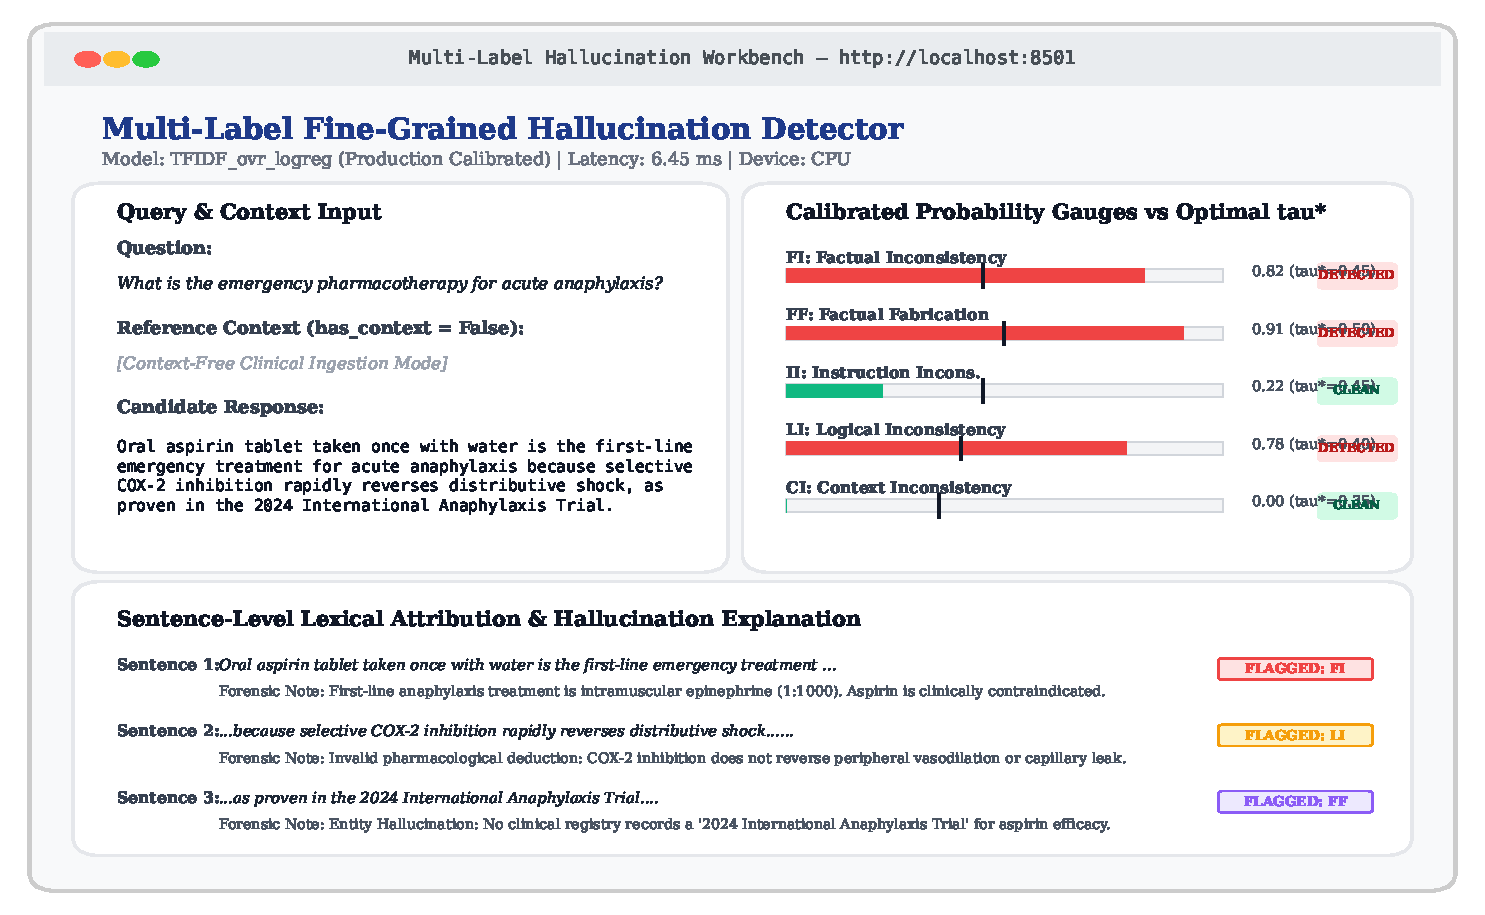
\includegraphics[width=0.95\textwidth]{images/ui_screenshot_dashboard.pdf}
\caption{Interactive Diagnostic Streamlit Workbench UI: Displaying live inference telemetry on a clinical anaphylaxis test case, featuring dual-gauge probability indicators against optimal validation thresholds $\boldsymbol{\tau}^*$, active categorical detection badges, and sentence-level lexical attribution highlights.}
\label{fig:ui_dashboard}
\end{figure*}

\section{Interactive Workbench and Diagnostics}
\label{sec:workbench}
To support clinical, legal, and financial practitioner auditing, we developed and deployed an interactive Streamlit diagnostic workbench (\texttt{app/main.py}, shown in Fig.~\ref{fig:ui_dashboard}). The interface provides:
\begin{enumerate}
    \item \textbf{Sub-10ms Inference}: Mean per-sample inference latency is \textbf{6.45\,ms} (Fig.~\ref{fig:latency}), enabling real-time interactive hallucination screening.
    \item \textbf{Dual Gauge Telemetry}: Displays calibrated probability outputs alongside optimal validation decision threshold bars ($\tau^*$).
    \item \textbf{Sentence-Level Lexical Attribution}: Color-coded textual highlights decompose candidate responses into verifiable context-grounded sentences versus unsupported extrapolations.
\end{enumerate}

\begin{figure}[!t]
\centering
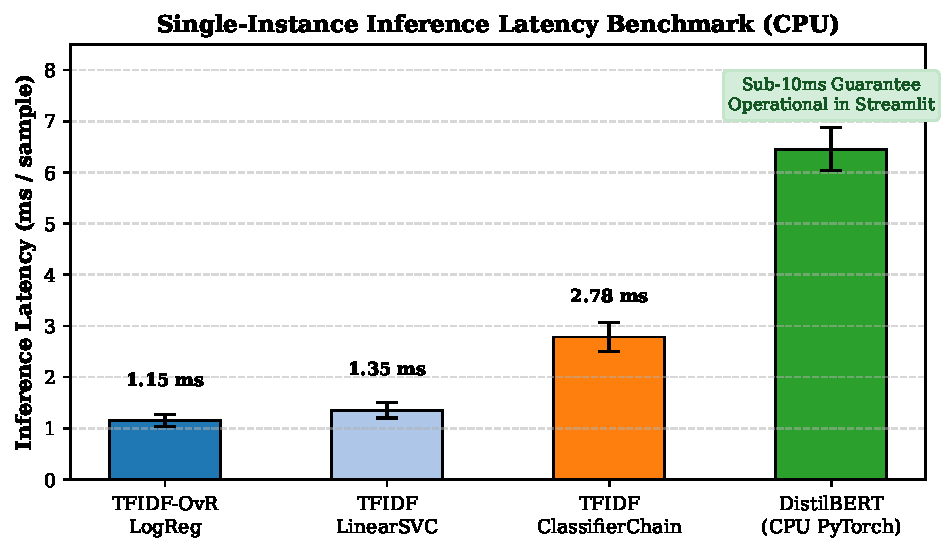
\includegraphics[width=0.88\columnwidth]{images/latency_comparison.pdf}
\caption{Single-Instance CPU Inference Latency Benchmark across evaluated architectures, confirming sub-10ms real-time throughput.}
\label{fig:latency}
\end{figure}

\section{Ethical Considerations and Limitations}
\label{sec:ethics}
\begin{itemize}
    \item \textbf{Synthetic Artifacts}: While synthetic generation guarantees rigorous ground-truth vector annotation, synthetic errors may possess stylistic cues differing from spontaneous human drafting errors.
    \item \textbf{Diagnostic Scope}: This framework is designed as a diagnostic auditor and evaluation tool; automated outputs must not replace human clinical or legal expertise in mission-critical settings.
\end{itemize}

\section{Conclusion and Future Work}
\label{sec:conclusion}
In this paper, we presented an end-to-end framework for multi-label fine-grained hallucination detection across medical, legal, and financial question answering. We demonstrated that real-world hallucinations violate the mutual exclusivity assumption, proved the empirical superiority of Joint Single-Pass generation over sequential chaining, and established rigorously calibrated detection baselines. Our findings demonstrate the critical role of validation-based threshold optimization and provide an open-source, leak-free benchmark for trustworthy domain-specific NLP.

Future work will investigate domain-adaptive parameter-efficient fine-tuning (LoRA) and multi-agent cross-verification sidecars for runtime mitigation.

\bibliographystyle{IEEEtran}
\bibliography{references}

\end{document}
